\documentclass[a4paper, 7pt, landscape]{scrartcl}
\usepackage[german]{babel}
\usepackage[utf8]{inputenc}
\usepackage{multicol}
\usepackage{geometry}
\usepackage{graphicx}
\usepackage{wrapfig}
\usepackage{enumitem}
\usepackage{fancyhdr}
\usepackage{index}
\usepackage{sectsty}
\usepackage{mwe}
\usepackage{comment}
\usepackage{lipsum}
\usepackage{titlesec}
\usepackage[dvipsnames]{xcolor}
\usepackage{amsmath}
\usepackage{amssymb}
\usepackage{listings}

%Define Math Commands:
\newcommand*{\field}[1]{\mathbb{#1}}%
\newcommand{\Mod}[1]{\ (\mathrm{mod}\ #1)}

%Image Folder:
\graphicspath{{./img/}}

%format
\geometry{top=0.4cm,left=0.5cm,right=0.5cm,bottom=0.4cm}
\setlist{topsep=0pt, leftmargin=5mm, nolistsep}

% Code Snippets

\definecolor{javared}{rgb}{0.6,0,0} % for strings
\definecolor{javagreen}{rgb}{0.25,0.5,0.35} % comments
\definecolor{javapurple}{rgb}{0.5,0,0.35} 

\lstset{
language=Java,
basicstyle=\fontsize{7}{7} \ttfamily,
keywordstyle=\bfseries\color{javapurple},
stringstyle=\color{javared},
commentstyle=\color{javagreen},
morecomment=[s][\color{MidnightBlue}]{/**}{*/},
tabsize=2,
showspaces=false,
showstringspaces=false,
texcl = true,
rulecolor = \color{black},
breaklines = true,
aboveskip = 0.5em,
belowskip = 0em
}




% Define Section Format
\titleformat{name=\section}[block]
{\sffamily\normalsize}
{}
{0pt}
{\colorsection}
\titlespacing*{\section}{0pt}{3pt}{3pt}

\newcommand{\colorsection}[1]{%
\colorbox{MidnightBlue!40}{\parbox{0.98\linewidth}{\color{black}\thesection\ #1}}}


% Define Subsection Format
\titleformat{name=\subsection}[block]
{\sffamily\small}
{}
{0pt}
{\colorsubsection}
\titlespacing*{\subsection}{0pt}{3pt}{3pt}

\newcommand{\colorsubsection}[1]{%
\colorbox{YellowGreen!50}{\parbox{0.98\linewidth}{\color{black}\thesubsection\ #1}}}

% Define SubSubsection Format
\titleformat{name=\subsubsection}[block]
{\sffamily\small}
{}
{0pt}
{\colorsubsubsection}
\titlespacing*{\subsubsection}{0pt}{3pt}{3pt}

\newcommand{\colorsubsubsection}[1]{%
\colorbox{Goldenrod!50}{\parbox{0.98\linewidth}{\color{black}\thesubsubsection\ #1}}}

% -----------------------------------------------------------------------
\begin{document}
    %	\pagecolor{p}
    %	\color{t}
    \setlength{\columnseprule}{0.4pt}
    \footnotesize
    \begin{multicols*}{2}

        %! Author = Philipp Emmenegger
%! Date = 30/06/2021

\section{Einführung}
\textbf{Nutzen ComBau}
\begin{itemize}
    \item Programmiersprachen und Sprachkonzepte besser verstehen
    \item Sprachfeatures beurteilen können
    \item Konzepte in verwandten Bereichen einsetzen
\end{itemize}

\subsection{Begriffe}
\textbf{Compiler}
\begin{itemize}
    \item Transformiert Quellcode in Maschinencode
\end{itemize}
\textbf{Runtime System}
\begin{itemize}
    \item Unterstützt die Programmausführung mit Software und Hardware Mechanismen
\end{itemize}
\textbf{Syntax}
\begin{itemize}
    \item Definiert Struktur des Programms
    \item Bewährte Formalismen für Syntax
\end{itemize}
\textbf{Semantik}
\begin{itemize}
    \item Definiert Bedeutung des Programms
    \item Meist in Prosa beschrieben
\end{itemize}

\subsection{Architekturen}
\begin{center}
    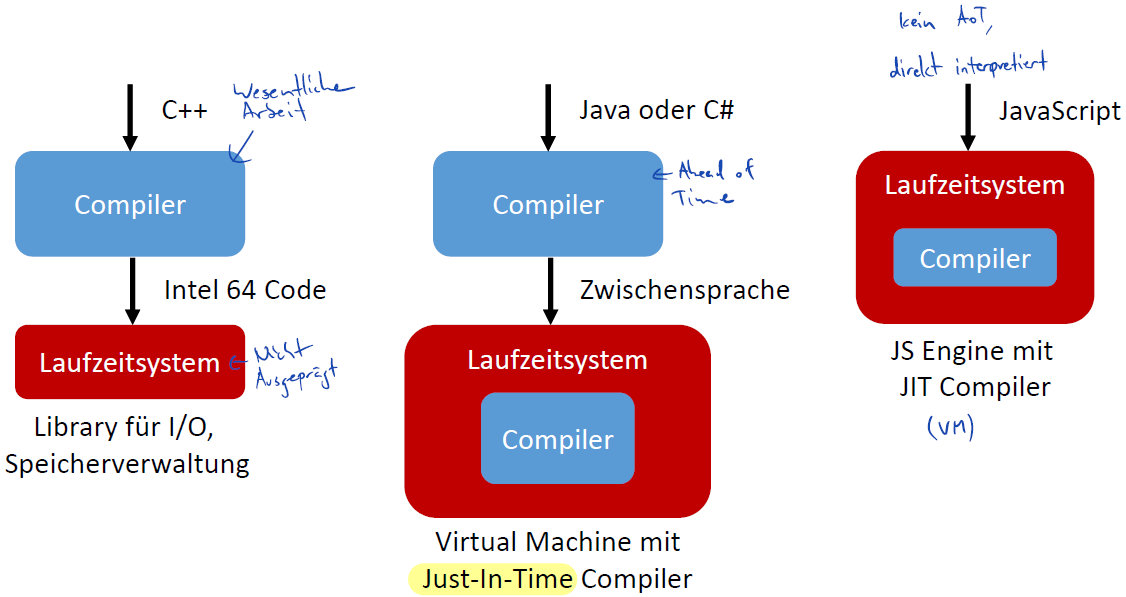
\includegraphics[width=0.6\linewidth]{/architekturen.png} 
\end{center}

\subsection{Aufbau Compiler}
\begin{center}
    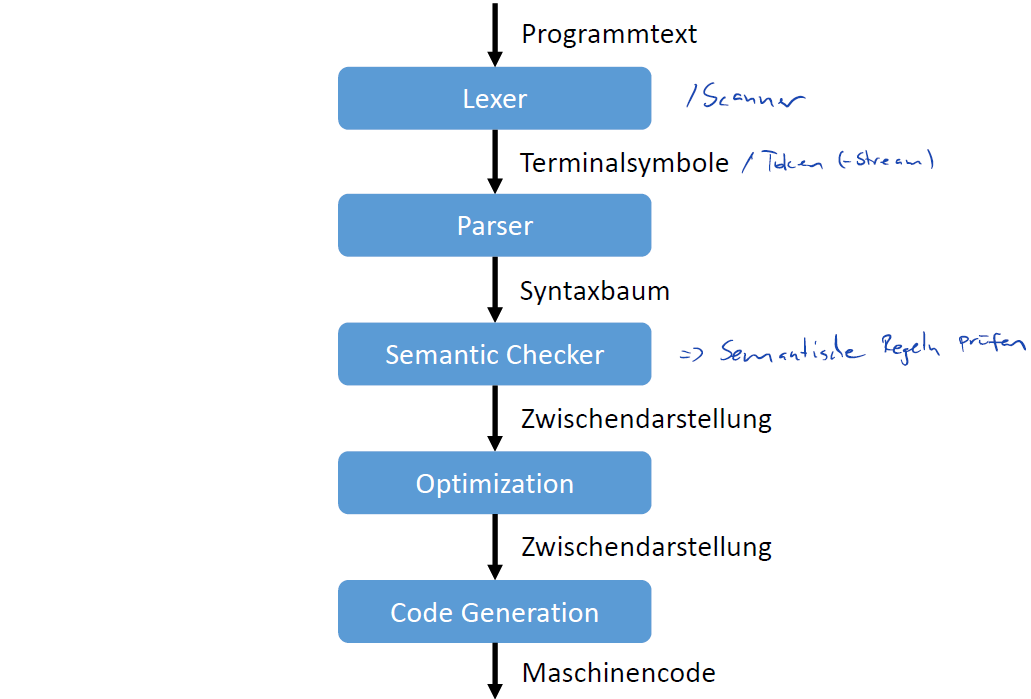
\includegraphics[width=0.5\linewidth]{/aufbau_compiler.png} 
\end{center}
\subsubsection{Lexer}
\textbf{Lexikalische Analyse, Scanner}
\begin{itemize}
    \item Zerlegt Programmtext in Terminalsymbole (Tokens)
    \item keine Tiefenstruktur
\end{itemize}
\subsubsection{Parser}
\textbf{Syntaktische Analyse}
\begin{itemize}
    \item Erzeugt Syntaxbaum gemäss Programmstruktur
    \item Kontextfreie Sprache
\end{itemize}
\subsubsection{Semantic Checker}
\textbf{Semantische Analyse}
\begin{itemize}
    \item Löst Symbole auf
    \item Prüft Typen und semantische Regeln
\end{itemize}
\subsubsection{Optimization}
\begin{itemize}
    \item Wandelt Zwischendarstellung in effizientere um
\end{itemize}
\subsubsection{Code Generation}
\begin{itemize}
    \item Erzeugt ausführbarer Maschinencode
\end{itemize}
\subsubsection{Zwischenarstellung}
\textbf{Intermediate Representation}
\begin{itemize}
    \item Beschreibt Programm als Datenstruktur (diverse Varianten)
\end{itemize}

\subsection{Aufbau Laufzeitsystem}
\begin{center}
    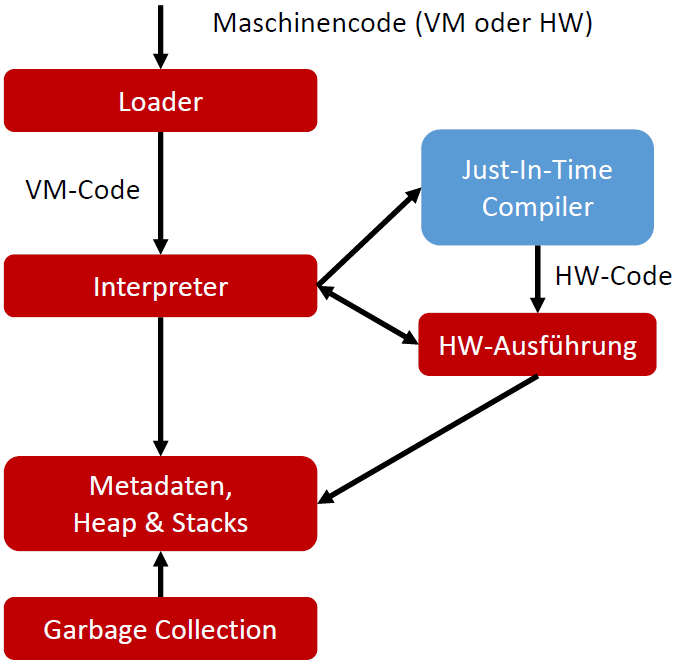
\includegraphics[width=0.4\linewidth]{/aufbau_laufzeitsystem.png} 
\end{center}
\subsubsection{Loader}
\begin{itemize}
    \item Lädt Maschinencode in Speicher
    \item Veranlasst Ausführung
\end{itemize}
\subsubsection{Interpreter}
\begin{itemize}
    \item Liest Instruktionen und emuliert diese in Software
\end{itemize}
\subsubsection{JIT (Just-In-Time) Compiler}
\begin{itemize}
    \item Übersetzt Code-Teile in Hardware-Instruktionscode
\end{itemize}
\subsubsection{HW-Ausführung (nativ)}
\begin{itemize}
    \item Lässt Instruktionscode direkt auf HW-Prozessor laufen
\end{itemize}
\subsubsection{Metadaten, Heap + Stacks}
\begin{itemize}
    \item Merken Programminfos, Objekte und Prozeduraufrufe
\end{itemize}
\subsubsection{Garbage Collection}
\begin{itemize}
    \item Räumt nicht erreichbare Objecte ab
\end{itemize}
\newpage

\subsection{Syntax}
\subsubsection{EBNF}
\textbf{Extended Backus-Naur Form}
\begin{center}
    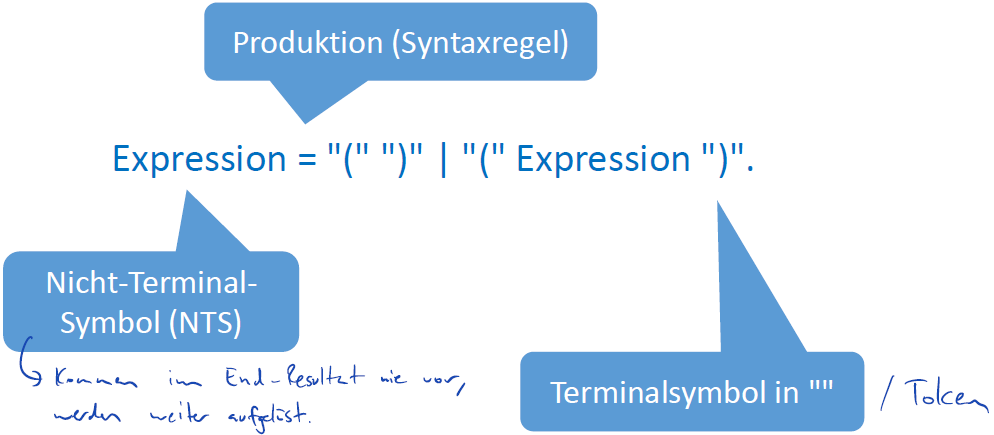
\includegraphics[width=0.5\linewidth]{/ebnf.png} 
    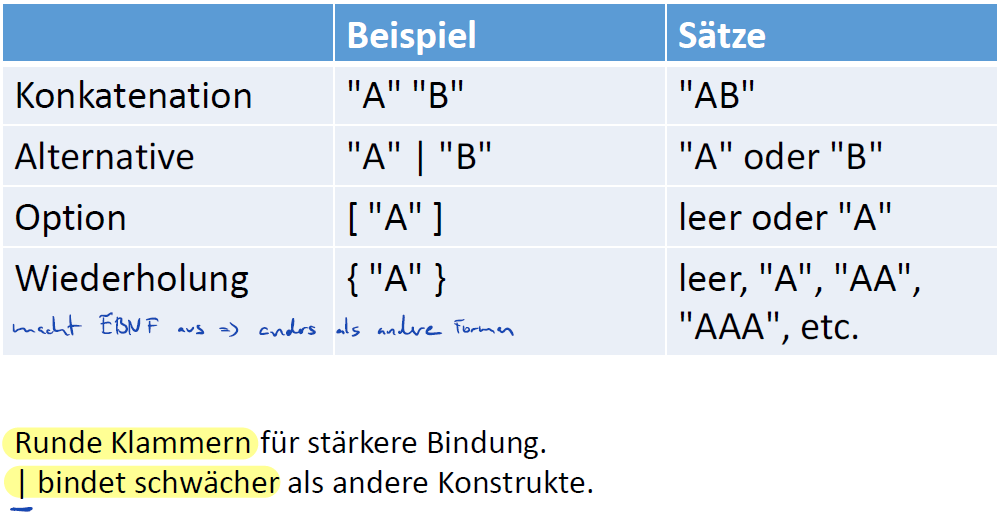
\includegraphics[width=0.5\linewidth]{/ebnf_regeln.png} 
\end{center}
\subsubsection{Arithmetische Ausdrücke}
\begin{center}
    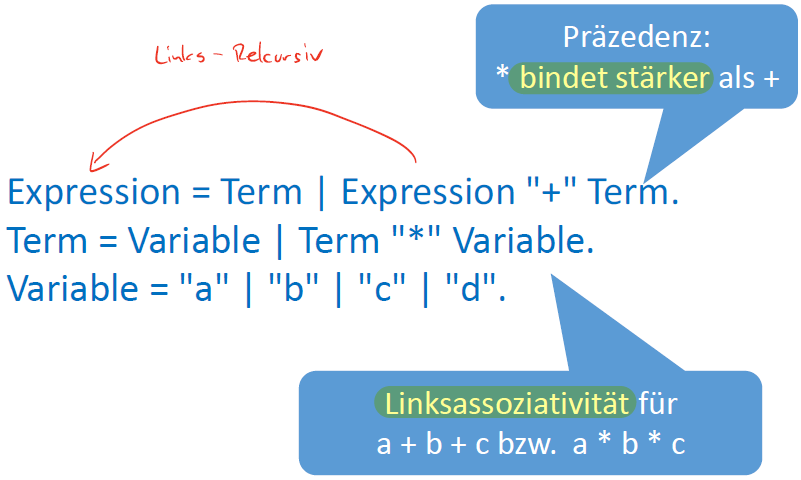
\includegraphics[width=0.5\linewidth]{/ebnf_arithmetisch.png} 
\end{center}
        \newpage
        \section{Lexikalische Analyse}
\subsection{Lexer / Scanner}
\textbf{Endlicher Automat (DEA)}
\begin{itemize}
    \item Kümmert sich um die lexikalische Analyse
    \item Input: Zeichenfolge (Programmtext)
    \item Output: Folge von Terminalsymbolen (Tokens)
\end{itemize}
\subsubsection{Aufgaben}
\begin{itemize}
    \item Fasst Textzeichen zu tokens zusammen
    \item Eliminiert Whitespaces
    \item Eliminiert Kommentare
    \item Merkt Positionen in Programmcode
\end{itemize}
\subsubsection{Nutzen}
\textbf{Abstraktion}
\begin{itemize}
    \item Parser muss sich nicht um Textzeichen kümmern
\end{itemize}
\textbf{Einfachheit}
\begin{itemize}
    \item Parser braucht Lookahead pro Symbol, nicht Textzeichen
\end{itemize}
\textbf{Effizienz}
\begin{itemize}
    \item Lexer benötigt keinen Stack im Gegensatz zu Parser
\end{itemize}

\subsection{Tokens}
\textbf{Statisch (Keywords, Operationen, Interpunktion)}
\begin{itemize}
    \item \textit{if}
    \item \textit{else}
    \item \textit{while}
    \item \textit{*}
    \item \textit{\&\&}
    \item \textit{;}
\end{itemize}
\textbf{Identifiers}
\begin{itemize}
    \item MyClass
    \item readFile
    \item name2
\end{itemize}
\textbf{Zahlen}
\begin{itemize}
    \item 123
    \item 0xfe12
    \item 1.2e-3
\end{itemize}
\textbf{Strings}
\begin{itemize}
    \item \dq Hello\dq
    \item \dq \dq
    \item \dq $\backslash$n\dq
\end{itemize}
\begin{center}
    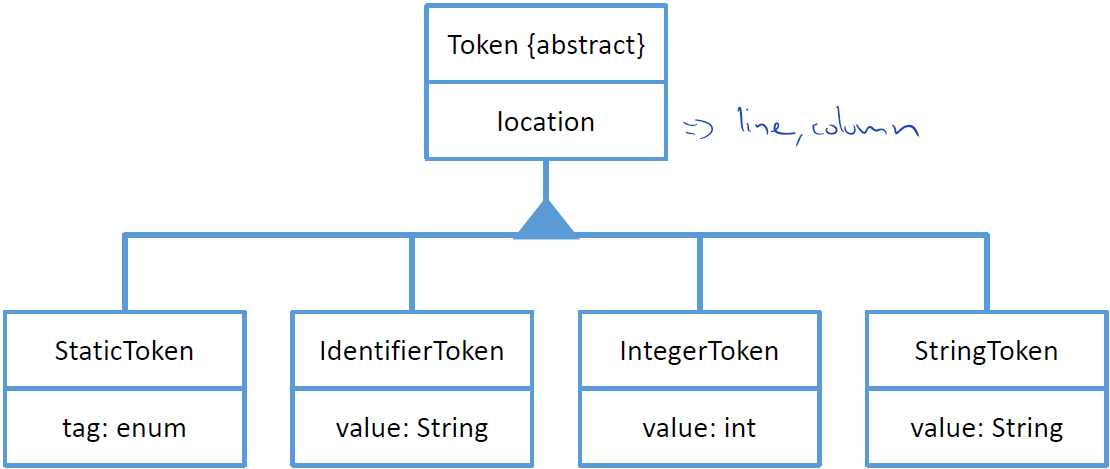
\includegraphics[width=0.4\linewidth]{/token_model.png} 
\end{center}

\subsubsection{Lexem}
\begin{itemize}
    \item Spezifische Zeichenfolge, die einen Token darstellt
    \item z.B. \textit{MyClass} ist ein Lexem des Tokens Identifier
\end{itemize}

\subsubsection{Maximum Munch}
\begin{itemize}
    \item Lexer absorbiert möglichst viel in einem Token
\end{itemize}

\subsection{Reguläre Sprachen}
\begin{itemize}
    \item Lexer unterstützt nur reguläre Sprachen
    \item \textbf{Regulär:} Als EBNF ohne Rekursion ausdrückbar
\end{itemize}
\begin{center}
    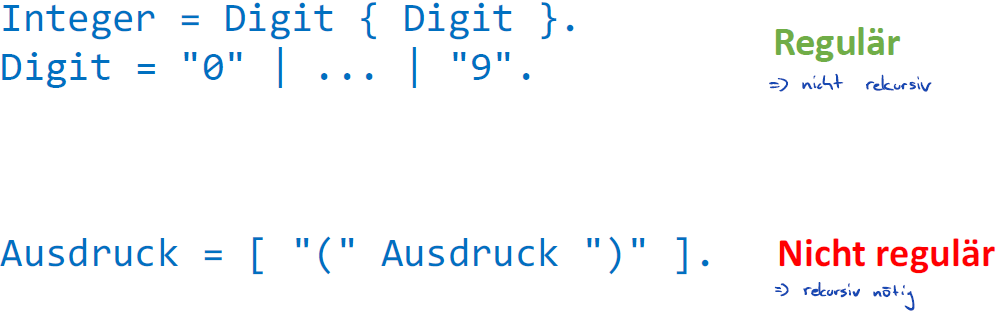
\includegraphics[width=0.5\linewidth]{/reg_sprachen.png} 
\end{center}

\subsection{Chomsky Hierarchie}
\begin{center}
    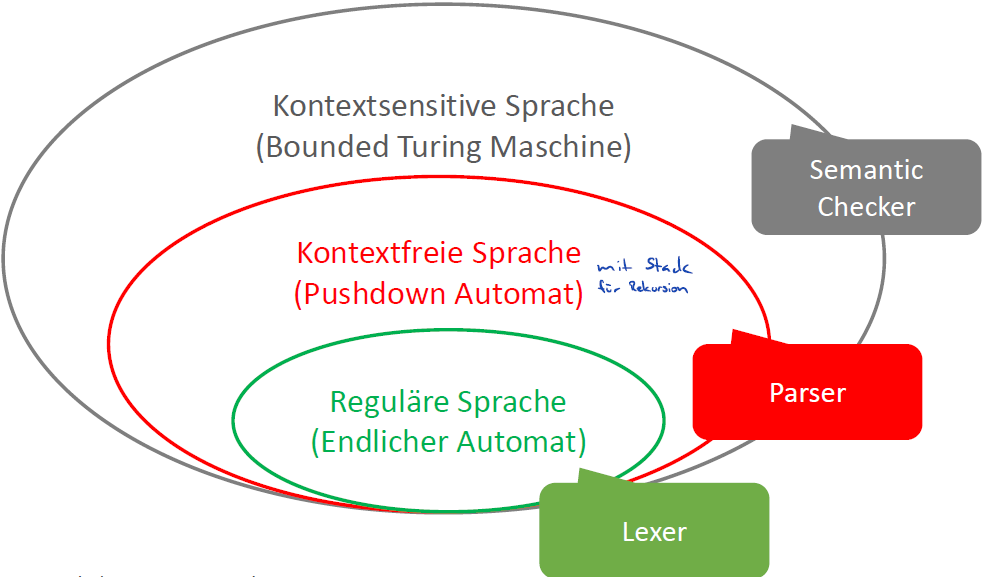
\includegraphics[width=0.7\linewidth]{/chomsky.png} 
\end{center}

\subsection{Lexer Gerüst}
\begin{lstlisting}
class Lexer {
    private final Reader reader;
    private char current; // one Character Lookahead
    private boolean end; // EOF 

    private Lexer(Reader reader) {
        this.reader = reader;
    }

    public static Iterable<Token> scan(Reader reader) {
        return new Lexer(reader).readTokenStream();
    }

    // ...
}
\end{lstlisting}

\subsection{Token Stream lesen}
\begin{lstlisting}
Iterable<Token> readTokenStream() {
    var stream = new ArrayList<Token>();
    readNext(); // One Character Lookahead
    skipBlanks();
    while (!end) {
        stream.add(readToken());
        skipBlanks();
    }
    return stream;
}
\end{lstlisting}

\subsection{Lexer Kernlogik}
\begin{lstlisting}
Token readToken() {
    if(isDigit(current)) {
        return readInteger();
    }
    if(isLetter(current)) {
        return readName(); // Identifier / Keyword 
    }
    return switch(current) {
        case '"': readString();
        case '+': readStaticToken(Tag.Plus);
        case '-': readStaticToken(Tag.Minus);
        case '/': readPotentialSlash();
    }
}
\end{lstlisting}

\subsubsection{Static Token scannen}
\begin{lstlisting}
StaticToken readStaticToken(Tag tag) {
    readNext();
    return new StaticToken(tag);
}
\end{lstlisting}

\subsubsection{Zahlen scennen}
\textbf{Beachten:}
\begin{itemize}
    \item Range Check (32 bit): Integer Overflow
    \item $Integer.MIN$ = $Integer.MAX+1$
\end{itemize}
\begin{lstlisting}
IntegerToken readInteger() {
    int value = 0;
    while (!_end && isDigit(current)) {
        int digit = current - '0'; // char to int 
        value = value * 10 + digit; // create decimal number
        readNext();
    }
    return new IntegerToken(value);
}
\end{lstlisting}

\subsubsection{Identifier und Keywords scannen}
\begin{lstlisting}
Token readName() {
    String name = Character.toString(current);
    readNext();
    while(!end & (isLetter(current) || isDigit(current))) {
        name += current;
        readNext();
    }
    if(KEYWORDS.containsKey(name)) {
        return new StaticToken(KEYWORDS.get(name));
    }
    return new IdentifierToken(name);
}
\end{lstlisting}

\subsubsection{String scannen}
\textbf{Beachten:}
\begin{itemize}
    \item Kein $\backslash$t
    \item Kein $\backslash$\dq
    \item Kein $\backslash$n
    \item Keine mehrzeiligen Strings
\end{itemize}
\begin{lstlisting}
StringToken readString() {
    readNext(); // Skip leading double Quote
    String value = "";
    while (!end && current != '"') {
        value += current;
        readNext();
    }
    if(end) {
        // Error: String not closed
    }
    readNext(); // Skip trailing double Quote
    return new StringToken(value);
}
\end{lstlisting}

\subsubsection{Kommentare erkennen}
\begin{lstlisting}
StaticToken readPotentialSlash() {
    readNext();
    if(current == '/') {
        skipLineComment();
        // move on to next token
    } else if (current == '*') {
        skipCommentBlock();
        // move on to next token
    } else {
        return new StaticToken(Tag.Divide);
    }
}
\end{lstlisting}
        \newpage
        \section{Parser}
\textbf{Kontextfreie Sprache}
\begin{itemize}
    \item Kümmert sich um die syntaktische Analyse
    \item Input: Tokens (Terminalsymbole)
    \item Output: Syntaxbaum / Parse Tree
\end{itemize}
\subsection{Aufgabe}
\begin{itemize}
    \item Finde eindeutige Ableitung der Syntaxregeln, um einen gegebenen Input herzuleiten
    \item Analysiert die gesamte Syntaxdefinition (mit rekursiven Regeln)
    \item Erkennt, ob Eingabetext Syntax erfüllt
    \item Erzeugt Syntaxbaum
\end{itemize}
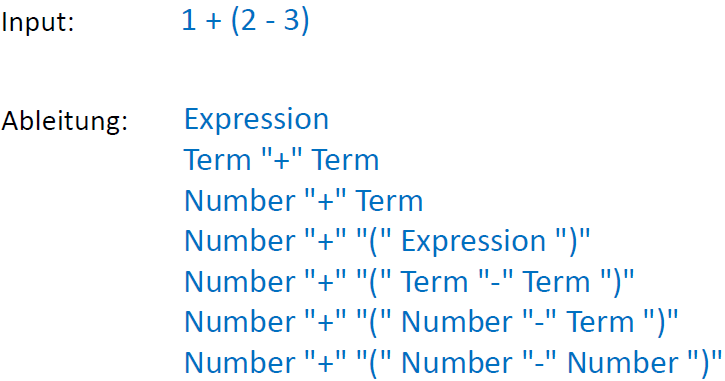
\includegraphics[width=0.5\linewidth]{/parser_aufgabe.png} 

\subsection{Parse Tree}
\begin{itemize}
    \item Concrete Syntax Tree
    \item Ableitung der Syntaxregeln als Baum wiedergespiegelt
    \item Kann generiert werden
\end{itemize}
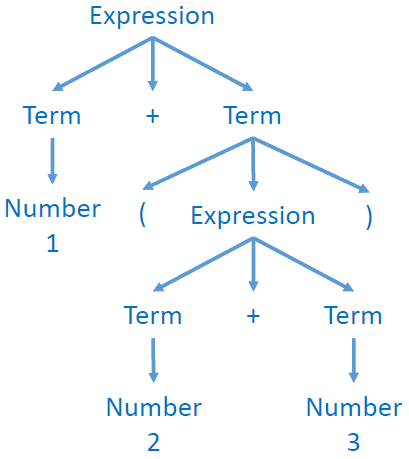
\includegraphics[width=0.3\linewidth]{/parse_tree.png} 

\subsubsection{Abstract Syntax Tree}
\begin{itemize}
    \item Unwichtige Details auslassen
    \item Struktur vereinfacht
    \item Für Weiterverarbeitung massgeschneidert
    \item Eigendesign nach Gusto des Compiler-Entwicklers
    \item Nur mit Selbstimplementation möglich
\end{itemize}
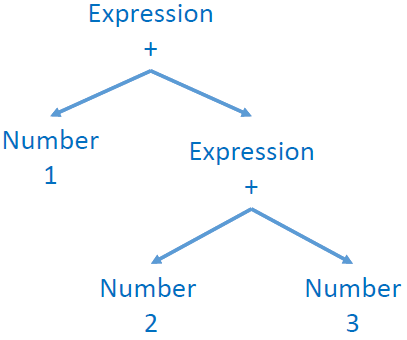
\includegraphics[width=0.3\linewidth]{/abstract_parse_tree.png} 

\subsection{Parser Strategien}
\subsubsection{Top-Down}
\begin{itemize}
    \item Beginne mit Start-Symbol
    \item Wende Produktionen an
    \item Expandiere Start-Symbol auf Eingabetext
    \item $Expr -> Term + Term -> ... -> 1 + (2 - 3)$
\end{itemize}
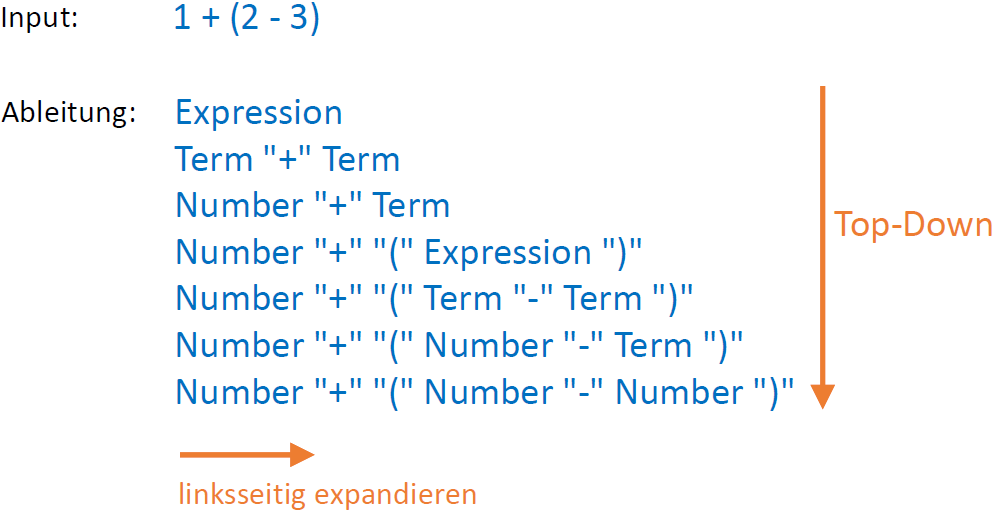
\includegraphics[width=0.5\linewidth]{/top_down.png} 

\subsubsection{Bottom-Up}
\begin{itemize}
    \item Beginne mit Eingabetext
    \item Wende Produktionen an
    \item Reduziere Eingabetext auf Start-Symbol
    \item $Expr <- Term + Term <- ... <- 1 + (2 - 3)$
\end{itemize}
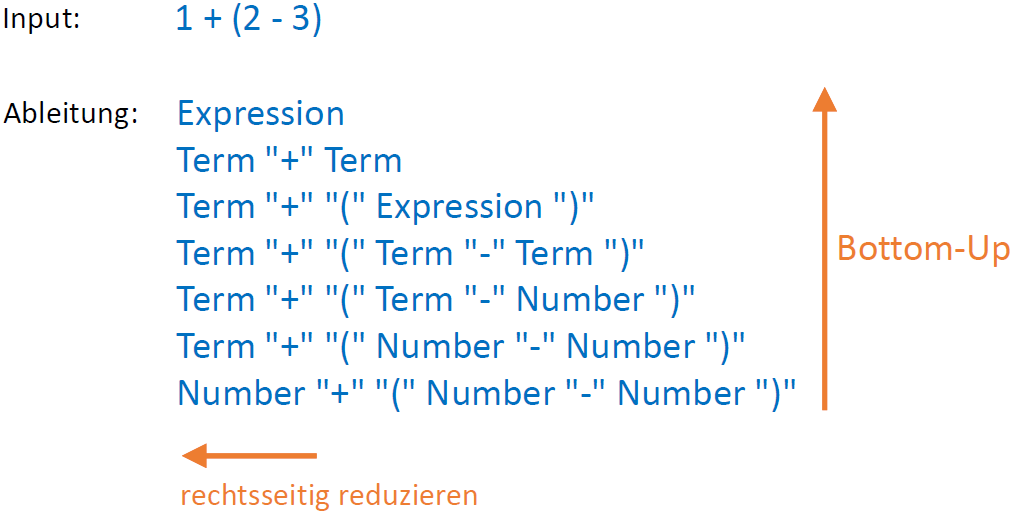
\includegraphics[width=0.5\linewidth]{/bottom_up.png} 

\subsection{Recursive Descent}
\begin{itemize}
    \item Pro Nicht-Terminalsymbol eine Methode
    \begin{itemize}
        \item Implementiert die Erkennung gemäss EBNF-Produktion
    \end{itemize}
    \item Vorkommen eines Nicht-Terminalsymbols in Syntax
    \begin{itemize}
        \item Aufruf der entsprechenden Methode
    \end{itemize}
    \item Funktioniert bei rekursiven und nicht-rekursiven Produktionen
\end{itemize}
\begin{lstlisting}
void parseExpression() {
    parseTerm();
    // ...
}
void parseTerm() {
    parseExpression();
    // ...
}
\end{lstlisting}

\subsection{Parser Gerüst}
\begin{lstlisting}
public class Parser {
    private final Iterator<Token> tokenStream;
    private Token current; // One Token Lookahead

    private Parser(Iterable<Token> tokenStream) {
        this.tokenStream = tokenStream.iterator();
    }

    public static ProgramNode parse(Iterable<Token> stream) {
        return new Parser(stream).parseProgram(); // Aufbasierte Klasse
    }
}
\end{lstlisting}

\subsubsection{Parser-Einstieg}
$Program = Expression$
\begin{lstlisting}
private ProgramNode parseProgram() {
    var classes = new ArrayList<ClassNode>();
    parseExpression();
    while (!isEnd()) {
        next();
        classes.add(parseClass());
    }
    return new ProgramNode(classes);
}
\end{lstlisting}

\subsubsection{Expression}
$Expression = Term { ( \dq +\dq | \dq -\dq ) Term }$
\begin{lstlisting}
Expression parseExpression() {
    var left = parseTerm();
    while(is(Tag.PLUS) || is(Tag.MINUS)) {
        var op = is(Tag.PLUS) ? Operator.PLUS : Operator.MINUS;
        next();
        var right = parseTerm();
        var left = new BinaryExpression(op, left, right);
    }
    return left;
}
\end{lstlisting}

\subsubsection{Term}
$Term = Number | \dq (\dq Expression \dq )\dq$
\begin{lstlisting}
Expression parseTerm() {
    if(isInteger()) {
        int value = readInteger();
        next();
        return new IntegerLiteral(value);
    } else if (is(Tag.OPEN_PARENTHESIS)) {
        next();
        var expression = parseExpression();
        if(is(Tag.CLOSE_PARENTHESIS)) {
            next();
        } else {
            error(); // missing closed parenthesis
        }
        return expression();
    } else {
        error(); // missing open parenthesis
    }
}
\end{lstlisting}

\subsection{One Symbol Lookahead}
\textbf{Statement}\\
$Assignment | IfStatement$
\begin{itemize}
    \item Bestimme mögliche Terminalsymbole, die mit einer Produktion ableitbar sind (FIRST-Menge)
    \item Benutze FIRST zur Entscheidung der Alternative beim zielorientierten Parsen
\end{itemize}
\begin{lstlisting}
void parseStatement() {
    if(isIdentifier()) { // FIRST(Assignment)
        parseAssignment();
    } else if(is(Tag.IF)) { // FIRST(IfStatement)
        parseIfStatement();
    } else {
        error();
    }
}
\end{lstlisting}

\subsection{Technische Syntax-Umformung}
\begin{itemize}
    \item Falls 1 Lookahead nicht reicht
\end{itemize}
\begin{lstlisting}
Statement = Assignment | Invocation
Assignment = Identifier "=" Expression
Invocation = Identifier "(" ")"
\end{lstlisting}

\begin{center}
    $\downarrow$
\end{center}

\begin{lstlisting}
Statement = Identifier (AssignmentRest | InvocationRest)
AssignmentRest = "=" Expression 
InvocationRest = "(" ")"
// Lookahead 1 reicht wieder
\end{lstlisting}

\subsubsection{Code Beispiel}
\begin{lstlisting}
var parseStatement() {
    var identifier = readIdentifier();
    next();
    if (is(Tag.ASSIGN)) {
        parseAssignmentRest(identifier);
    } else if (is(Tag.OPEN_PARENTHESIS)) {
        parseInvocationRest(identifier);
    } else {
        error();
    }
}
\end{lstlisting}
        \newpage
        \section{Parser Vertiefung}
\subsection{Abstrakter Syntaxbaum Design}
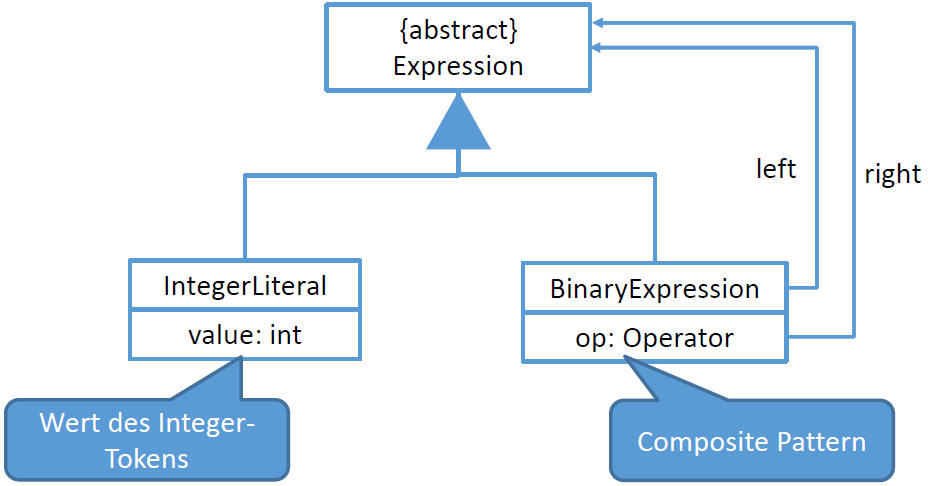
\includegraphics[width=0.7\linewidth]{syntaxbaum_design.png}

\subsection{Bottom-Up Parsing}
\begin{itemize}
    \item Mächtiger als LL (Top-Down) Parser
    \item Kann Linksrekursion behandeln
\end{itemize}
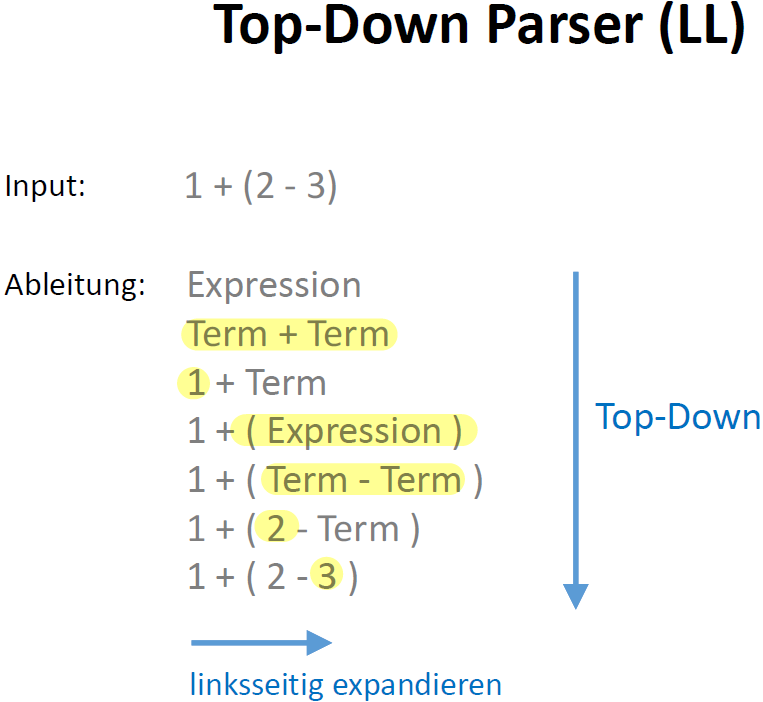
\includegraphics[width=0.5\linewidth]{top_down2.png}
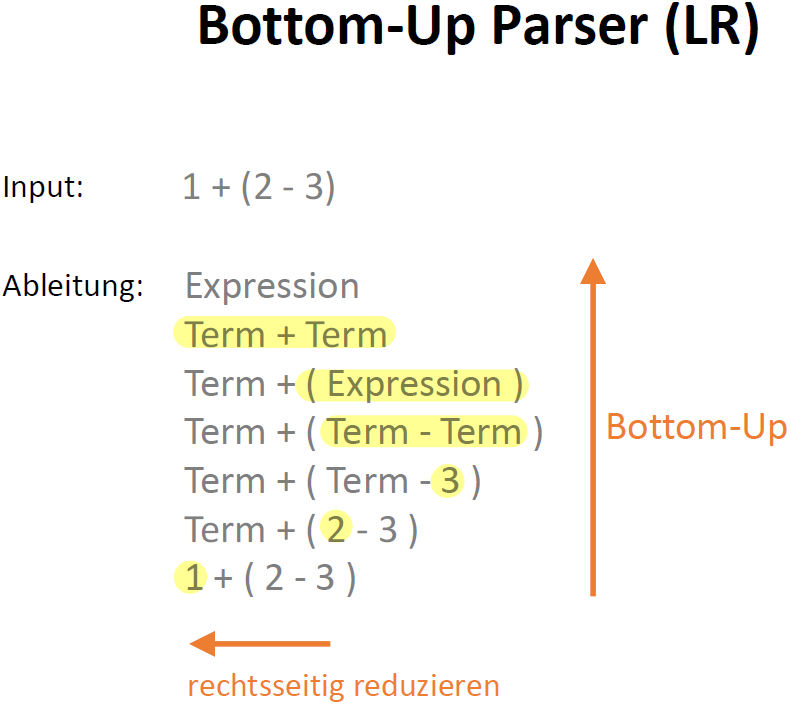
\includegraphics[width=0.5\linewidth]{bottom_up2.png}

\subsubsection{Ansatz}
\begin{itemize}
    \item Lese Symbole im Text ohne fixes Ziel
    \item Prüfe nach jedem Schritt, ob gelesene Folge Produktion entspricht
    \begin{itemize}
        \item Wenn ja: Reduziere auf Syntaxkonstrukt (REDUCE)
        \item Wenn nein: Lese weiteres Symbol im Text (SHIFT)
    \end{itemize}
    \item Am Schluss bleibt Startsymbol übrig, sonst Syntaxfehler
\end{itemize}

\subsubsection{Beispielablauf}
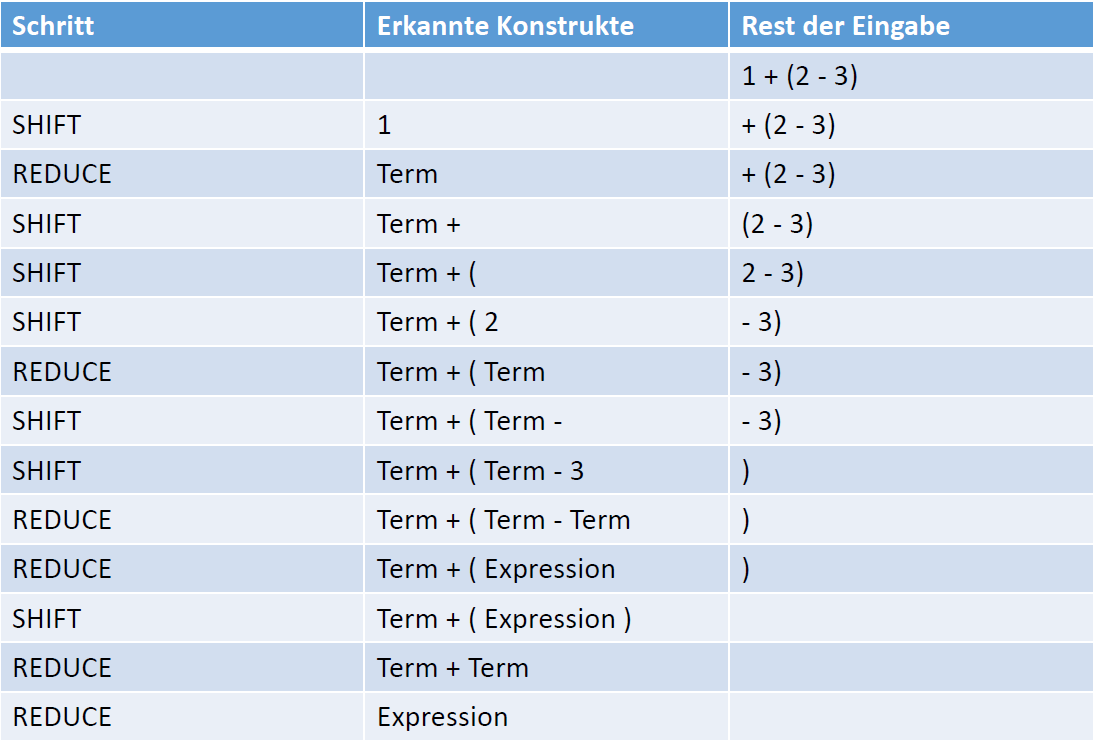
\includegraphics[width=0.7\linewidth]{bottom_up_ablauf.png}
\subsubsection{Parser Tabelle - Vereinfacht}
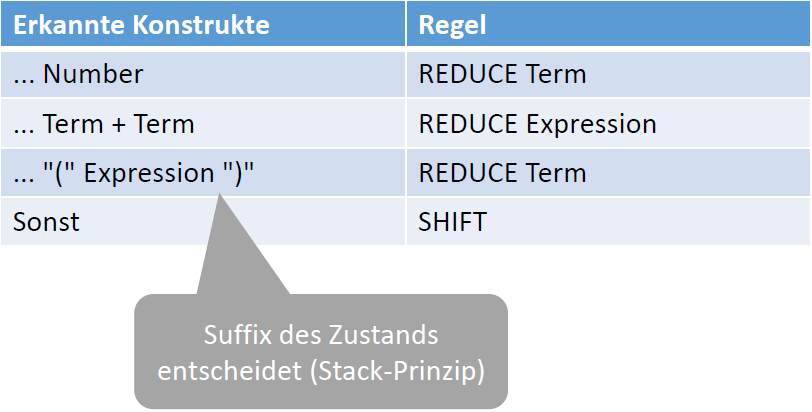
\includegraphics[width=0.5\linewidth]{parser_tabelle_vereinfacht.png}

\subsection{LR-Parser (Bottom-Up) Varianten}
\textbf{LR(0)}
\begin{itemize}
    \item Parse Tabelle ohne Lookahead erstellen
    \item Zustand reicht, um zu entscheiden
\end{itemize}
\textbf{SLR(k) (Simple LR)}
\begin{itemize}
    \item Lookahead bei REDUCE, um Konflikt zu lösen
    \item Keine neuen Zustände
\end{itemize}
\textbf{LALR(k) (Look-Ahead LR)}
\begin{itemize}
    \item Analysiert Sprache auf LR(0)-Konflikte
    \item Benutzt Lookahead bei Konfliktstellen mit neuen Zuständen
\end{itemize}
\textbf{LR(k)}
\begin{itemize}
    \item Pro Grammatikschritt + Lookahead ein Zustand
    \item Nicht praxistauglich, zu viele Zustände
\end{itemize}
        \newpage
        \section{Semantic Checker}
\begin{itemize}
    \item Kümmert sich um die semantische Analyse
    \item Input: Syntaxbaum
    \item Output: Zwischendarstellung (Syntaxbaum + Symboltabelle)
\end{itemize}
\subsection{Semantische Prüfung}
\textbf{Deklarationen}
\begin{itemize}
    \item Jeder Identifier ist eindeutig deklariert
\end{itemize}
\textbf{Typen}
\begin{itemize}
    \item Typregeln sind erfüllt
\end{itemize}
\textbf{Methodenaufrufe}
\begin{itemize}
    \item Argumente und Parameter sind kompatibel
\end{itemize}
\textbf{Weitere Regeln}
\begin{itemize}
    \item z.B. keine zyklischen Vererbung
    \item nur eine main() Methode
\end{itemize}

\subsection{Symboltabelle}
\begin{itemize}
    \item Datenstruktur zur Verwaltung der Deklarationen
    \item Wiederspiegelt hierarchische Bereiche im Programm
\end{itemize}
\subsubsection{Design}
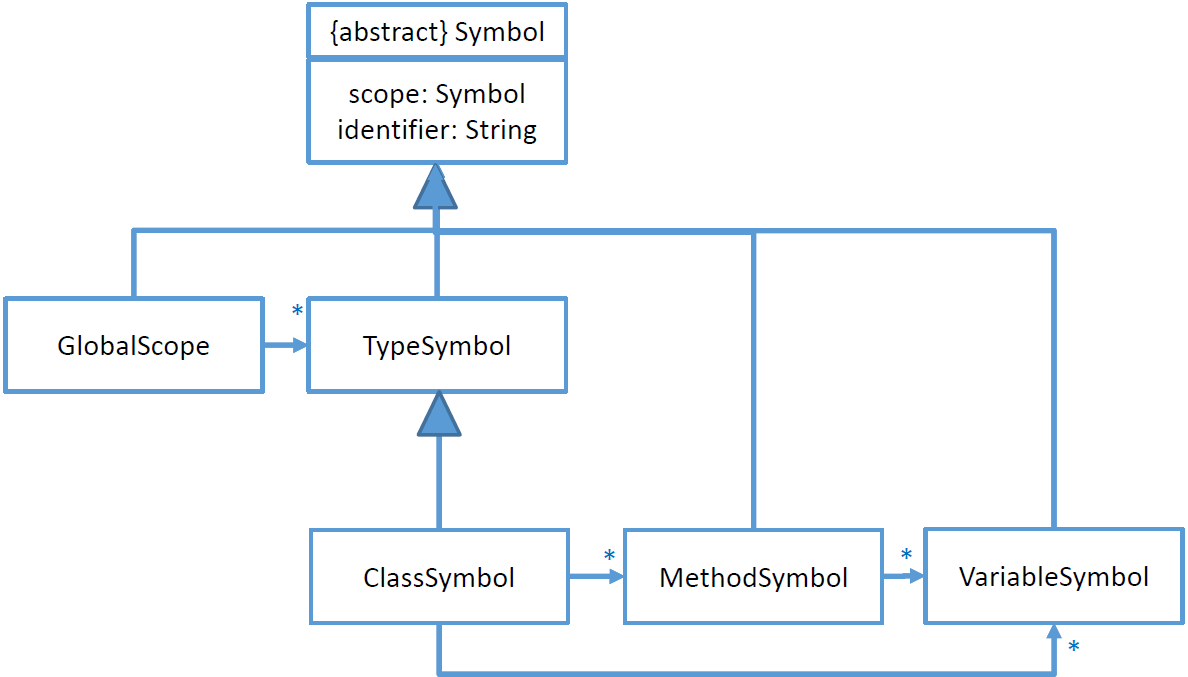
\includegraphics[width=0.7\linewidth]{symboltabelle_design.png}
\subsubsection{Detailiertere Beziehungen}
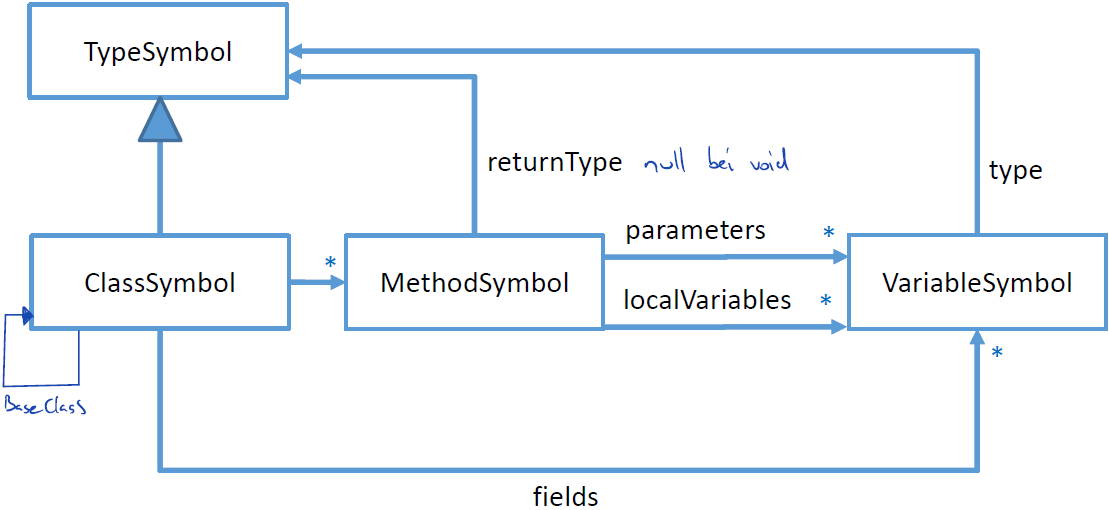
\includegraphics[width=0.7\linewidth]{symboltabelle_design_detailliert.png}
\subsubsection{Design Aspekte}
\textbf{Typinfo für Variable-Symbol}
\begin{itemize}
    \item Zuerst unaufgelöst (Identifier)
\end{itemize}
\textbf{Weitere Infos}
\begin{itemize}
    \item Klassen: Basisklasse
\end{itemize}
\textbf{Lokale Variablen}
\begin{itemize}
    \item Deklarationsbereich merken (Statements)
\end{itemize}
\textbf{Erweitertes Typ-Design}
\begin{itemize}
    \item Klassen
    \item Basistypen (int, boolean, string)
    \item Arrays
\end{itemize}
\textbf{Erweitertes Variablen-Design:}\\ 
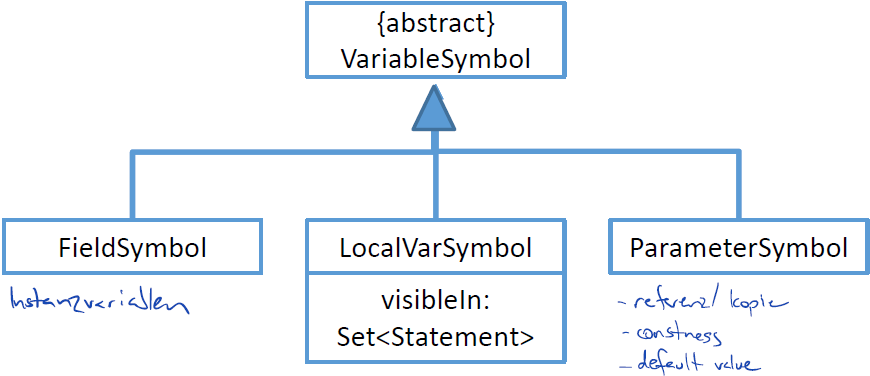
\includegraphics[width=0.5\linewidth]{var_design.png}
\subsubsection{AST Verknüpfung}
\begin{itemize}
    \item Symboltabelle enthält Mapping Symbol $\rightarrow$ AST
    \item Für alle Deklarationen
\end{itemize}
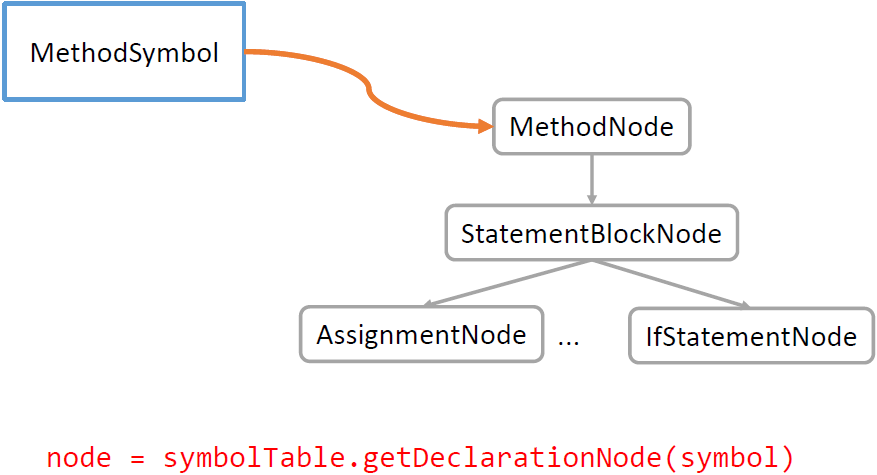
\includegraphics[width=0.6\linewidth]{ast_symboltabelle.png}

\subsection{Global Scope}
\begin{itemize}
    \item Mehrere Klassen im Programm
\end{itemize}

\subsection{Shadowing}
\begin{itemize}
    \item Deklarationen in inneren Bereichen verdecken gleichnamige von äusseren Bereichen
    \item Hiding: Bei gleicher Member-Name bei Vererbung
\end{itemize}

\subsection{Vorgehen}
\begin{enumerate}
    \item Konstruktion der Symboltabelle
    \item Typen in Tabelle auflösen 
    \item Deklaration in AST auflösen 
    \item Typen in AST auflösen
\end{enumerate}

\subsubsection{1. Konstruktion der Symboltabelle}
\textbf{AST traversieren}
\begin{itemize}
    \item Beginne mit Global Scope
    \item Pro Klasse, Methode, Parameter, Variable: Symbol in übergeordnetem Scope einfügen
    \item Explizit und/oder mit Visitor
\end{itemize}
\textbf{Forward-Referenzen $\rightarrow$ Typ-Namen und Designatoren noch nicht auflösen!}
\begin{itemize}
    \item Da vlt noch nicht alle Klassen in der Symboltabelle sind
\end{itemize}

\subsubsection{2. Typen in Tabelle auflösen}
\begin{itemize}
    \item Für Variablentype, Parametertyp, Rückgabetyp etc.
    \item Brauche Suche für Identifier auf Symboltabelle
    \begin{itemize}
        \item Starte mit innerstem Scope
        \item Suche stetig nach aussen ausbreiten
        \item Zuletzt in Global Scope suchen, ansonsten nicht vorhanden
    \end{itemize}
\end{itemize}
\begin{lstlisting}
Symbol find(Symbol scope, String identifier) {
    if(scope == null) {
        return null; // nicht im global scope
    }
    for (Symbol declaration : scope.allDeclarations()) {
        if(declaration.getIdentifier().equals(identifier)) {
            return declaration;
        }
    }
    return find(scope.getScope(), identifier); // rekursiv in nächst höheren Bereich
}
\end{lstlisting}

\subsubsection{3. Deklaration in AST auflösen}
\begin{itemize}
    \item Traversiere Ausführungscode in AST
    \item Jeden Designator auflösen, Deklaration zuordnen
\end{itemize}
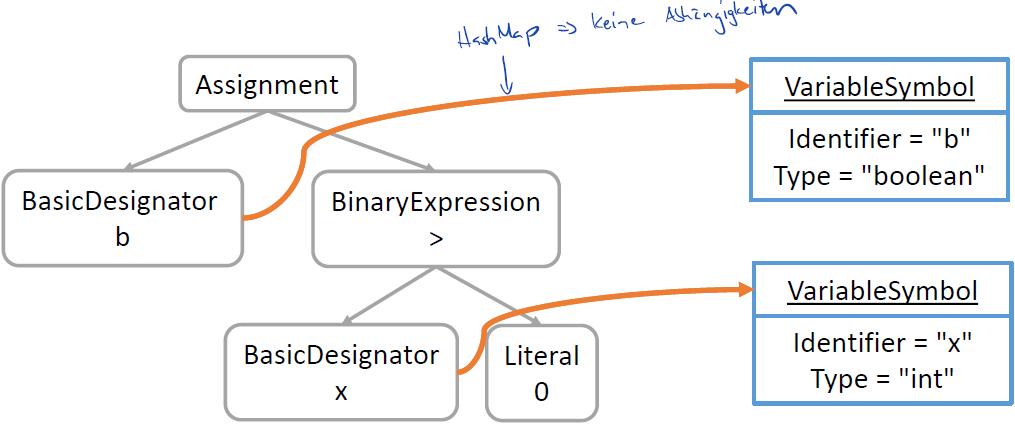
\includegraphics[width=0.7\linewidth]{dekl_in_ast.png}

\subsubsection{4. Typen in AST bestimmen}
\textbf{Typ zu jeder Expression zuordnen}
\begin{itemize}
    \item Literal: definierter Typ
    \item Designator: Typ der Deklaration
    \item Unary/BinaryExpression: Resultat des Operators
\end{itemize}
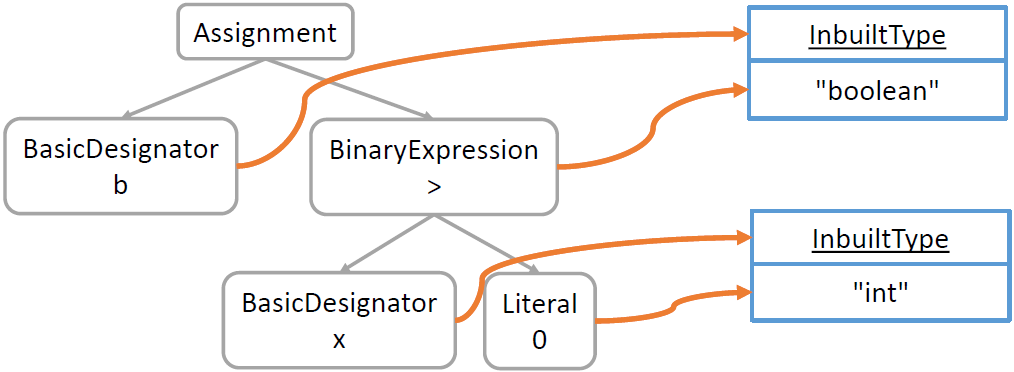
\includegraphics[width=0.7\linewidth]{typen_in_ast.png}\\
\textbf{Ablauf der Typenbestimmung:}
\begin{itemize}
    \item Post-Order-Traversierung
    \item AST am besten nicht erweitern sondern Maps in Symboltabelle verwenden
\end{itemize}
\subsubsection{Typauflösung per Visitor}
\begin{lstlisting}
@Override
public void visit(BinaryExpressionNode node) {
    Visitor.super.visit(node); // post-order travers
    var leftType = symboltable.findType(node.getLeft());
    var rightType = symboltable.findType(node.getRight());
    // ... 
    switch(node.getOperator()) {
        case PLUS -> {
            checkType(leftType, globalScope.getIntType());
            checkType(rightType, globalScope.getIntType());
            symboltable.fixType(node, globalScope.getIntType());
        }
        // ...
    }
}
\end{lstlisting}

\subsection{Semantic Checks}
\begin{itemize}
    \item Alle Designatoren beziehen sich auf Variablen/Methoden
    \item Typen stimmen bei Operatoren
    \item Kompatible Typen bei Zuweisungen
    \item Argumentliste passt auf Parameterliste
    \item Bedingungen in if, while sind boolean
    \item Return Ausdruck passt
    \item Keine Mehrfachdeklaration
    \item Kein Identifier ist reservierts Keyword
    \item Exakt eine main() Methode
    \item Array length  is read-only
    \item Kein Exit ohne Return (ausser void)
    \item Lesen von unitialisierten Variablen
    \item Null-Dereferenzierung
    \item Ungültiger Array-Index
    \item Division by Zero
    \item Out of Memory bei new()
\end{itemize}
        \newpage
        \section{Code Generator}
\subsection{Aufgabe}
\textbf{Erzeugung von ausführbarem Maschinencode}
\begin{itemize}
    \item Input: Zwischendarstellung (Symboltabelle + AST)
    \item Output: Maschinencode
\end{itemize}
\textbf{Mögliche Zielmaschinen}
\begin{itemize}
    \item Reale Maschine, z.B. intel 64, ARM Prozessor
    \item VM, z.B. JVM, .NET CLI
\end{itemize}

\subsection{Unsere Zielmaschine}
\textbf{Kernkonzepte}
\begin{itemize}
    \item Virtueller Stack-Prozessor: keine Register
    \item Branch Instructions (Goto): Programmfluss steuern
    \item Metadaten
\end{itemize}

\subsection{Stack Prozessor}
\begin{itemize}
    \item Instruktionen benutzen Auswertungs-Stack
    \item Keine Register wie auf echten Prozessoren
\end{itemize}

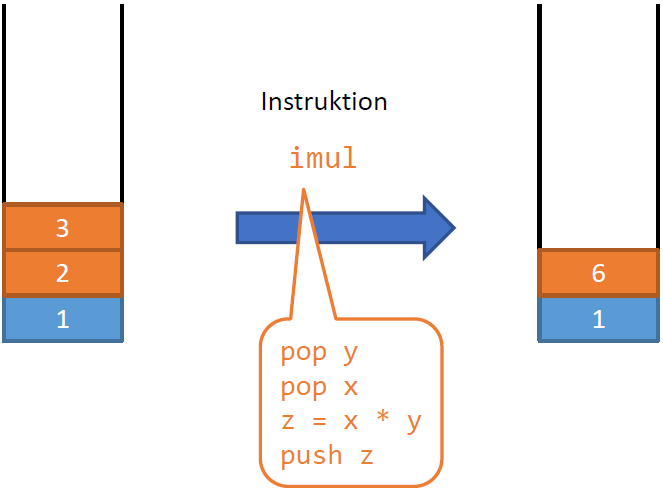
\includegraphics[width=0.5\linewidth]{stack_prozessor.png}

\subsection{Auswertungs-Stack}
\begin{itemize}
    \item Jede Instruktion hat definierte Anzahl von Pop- und Push-Aufrufen
    \item Eigener Stack pro Methodenaufruf
    \item Stack hat unbeschränkte Kapazität
\end{itemize}
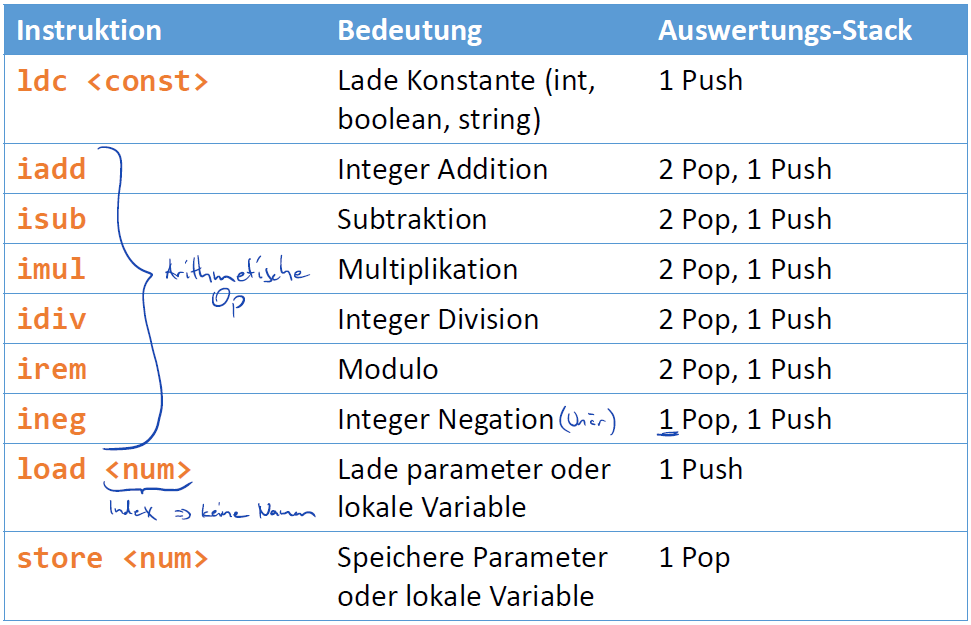
\includegraphics[width=0.5\linewidth]{instruktionen.png}

\subsubsection{Load/Store Nummerierungen}
\begin{itemize}
    \item \textit{this} Referenz: Index 0
    \item Danach, $n$ \textbf{Parameters}: Index $1..n$
    \item Danach, $m$ \textbf{lokale Variablen}: Index $n+1...n+m$
\end{itemize}
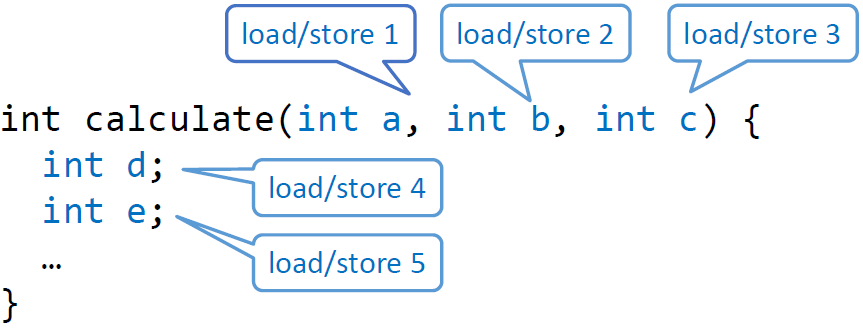
\includegraphics[width=0.5\linewidth]{load_store.png}

\subsubsection{Compare-Instruktionen}
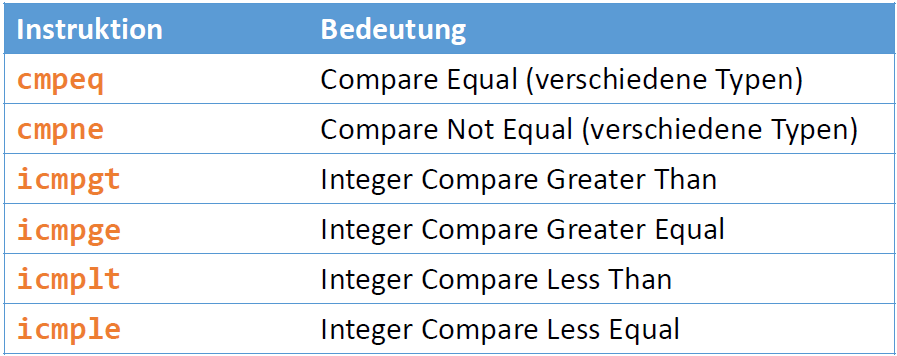
\includegraphics[width=0.5\linewidth]{compre_instruktionen.png}\\
\textbf{Pop right, Pop left, Push boolean}

\subsubsection{Branch-Instruktionen}
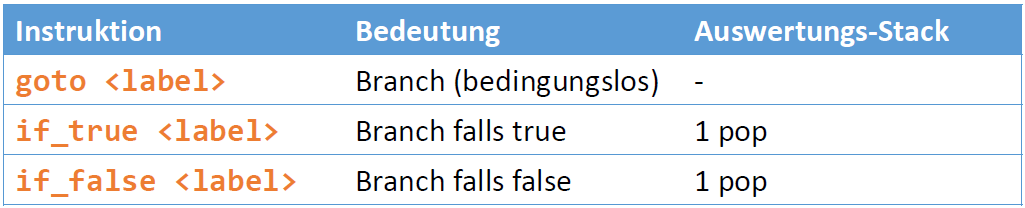
\includegraphics[width=0.5\linewidth]{branch_instruktionen.png}\\

\subsubsection{Metadaten}
\begin{itemize}
    \item Zwischensprache kennt alle Informationen zu
    \begin{itemize}
        \item Klassen (Namen, Typen der Fields und Methoden)
        \item Methoden (Namen, Parametertypen und Rückgabetyp)
        \item Lokale Variablen (Typen)
    \end{itemize}
    \item Kein direktes Speicherlayout festgelegt
    \item Nicht enthalten
    \begin{itemize}
        \item Namen von lokalen Variablen und Parameter
        \item Diese sind nur nummeriert
    \end{itemize}
\end{itemize}
\textbf{Verwendung:}
\begin{itemize}
    \item Speicherplatz-Allozierung
    \item Fehlermeldungen
    \item Funktionsaufrufe
\end{itemize}

\subsection{Code Generierung}
\begin{enumerate}
    \item Traversiere Symboltabelle: Erzeuge Bytecode Metadaten
    \item Traversiere AST pro Methode (Visitor): Erzeuge Instruktionen via Bytecode Assembler
    \item Serialisiere in Output Format
\end{enumerate}

\subsubsection{Backpatching}
\begin{itemize}
    \item Branch Offsets auflösen
    \item Label: relativer Instruktions-Offset ab Ende der aktuellen Branch-Instruktion
\end{itemize}

\subsubsection{Template-Basierte Generierung}
\begin{itemize}
    \item Postorder-Traversierung: Kinder zuerst besuchen
    \item Jeweils Template für erkanntes Teilbaum-Muster anwenden
\end{itemize}

\subsubsection{Short-Circuit Semantik}
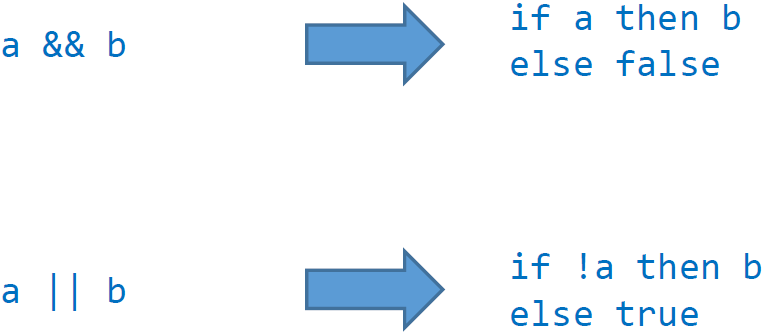
\includegraphics[width=0.5\linewidth]{short_circuit.png}

\subsubsection{Methodenaufruf}
\textbf{Statisch}
\begin{itemize}
    \item Vordefinierte Methoden: $readInt()$ etc.
\end{itemize}
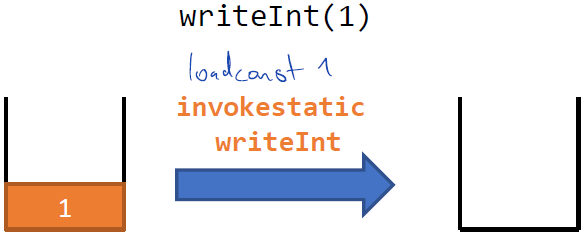
\includegraphics[width=0.4\linewidth]{static1.png}
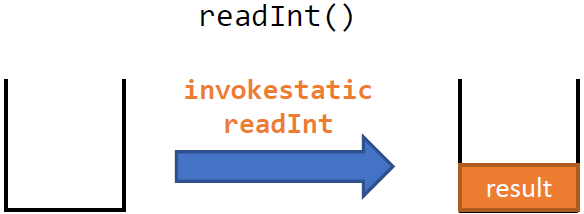
\includegraphics[width=0.4\linewidth]{static2.png}
\vspace{1cm}\\

\textbf{Virtuell}
\begin{itemize}
    \item Alle anderen Methoden
\end{itemize}
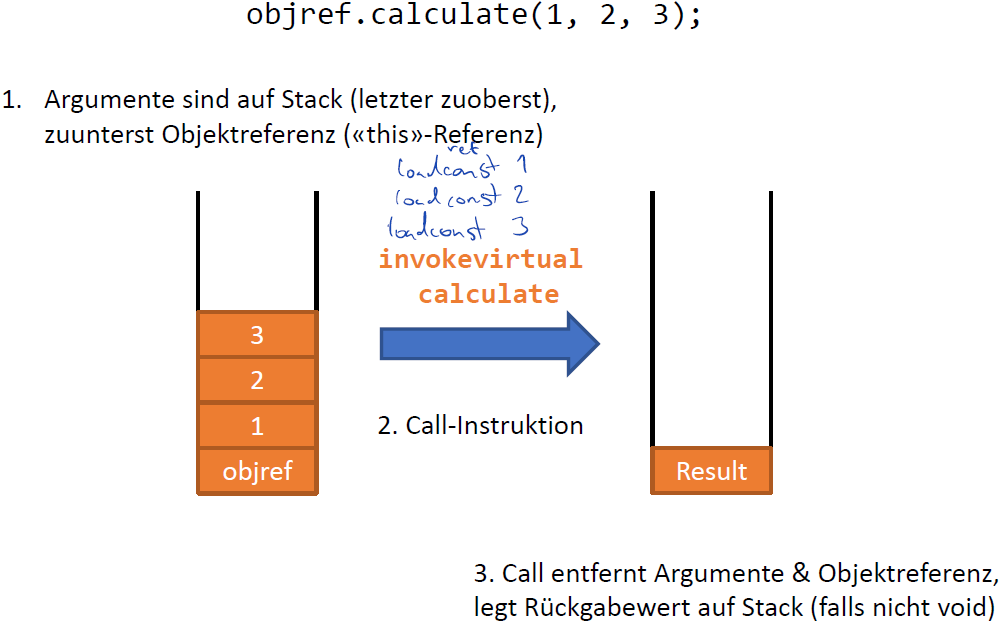
\includegraphics[width=0.5\linewidth]{virt.png}

\subsubsection{Parameter \& Rückgabe}
\begin{lstlisting}
int sum(int x, int y) {
    return x + y;
}

load 1 // load param x
load 2 // load param y
iadd // x + y
ret // return from method (auch bei void, max 1 Wert auf Stack)
\end{lstlisting}
        \newpage

    \end{multicols*}
\end{document}

























